{\let\clearpage\relax \chapter{表格}}

\section{浮动体}

在学习\LaTeX{}表格和图片的编排之前,了解一下什么是浮动体。\textbf{图片和表格有时会很大,在插入的位置不一定放得下,因此需要浮动调整,这样一个浮动调整的环境就成为浮动体。}

\note{因为有浮动体的存在,图片编排的位置是不确定的,所以要避免在文中使用「下图」、「上图」的说法,而是使用ref命令生成图表的编号。}

浮动体将图或表与其标题定义为整体,然后动态排版,以解决图、表卡在换页处造成的过长的垂直空白的问题。但有时它也会打乱你的排版意图,因此使用与否需要根据情况决定。图片的浮动体是figure环境,而表格的浮动体是table环境。

对表格来说,输出表格内容的是tabular环境,\textbf{table}只是一个会浮动体(到处乱跑的盒子)而已。没有tabular环境,table环境一样会乱跑;没有table环境,tabular环境一样会输出表格内容。图片浮动体与表格是一样的。图片和表格的浮动体环境如下所示:

\begin{latex}
\begin{table}[!htbp]
表格
\end{table}
%%%%%%%%%%%%%%%%%%%%
\begin{figure}[!htbp]
图片
\end{figure}
\end{latex}

!表示忽略内部参数(比如内部参数对一页中浮动体数量的限制);h当前位置(here),t顶部(top),b底部(bottom),p单独成页(p)。\LaTeX{}的默认参数是tbp。另外需要注意的是label命令写在caption命令下方,否则交叉引用会出现问题。

\section{array宏包}

数组宏包\emph{array}改进和扩展了\LaTeX 的\emph{tabular、tabular*、array}环境的功能,增强了\emph{列格式}的功能和一些其他表格参数的调整功能。

\begin{table}[!ht]
    \caption{array宏包基本参数}
    \begin{center}
    \begin{tabular}{|c|c|}
    \hline 
    选项    &    说明 \\ 
    \hline
    l    &    左对齐 \\ 
    \hline
    c    &    居中 \\ 
    \hline
    r    &    右对齐 \\ 
    \hline
    p\{列宽\}    &    顶对齐 \\ 
    \hline
    m\{列宽\}    &    居中对齐 \\ 
    \hline
    b\{列宽\}    &    底对齐 \\ 
    \hline
    @\{声明\}    &    该列每行都插入声明中的文本 \\ 
    \hline
    >\{声明\}    &    命令或需要插入列元素前的文本 \\ 
    \hline
    <\{声明\}    &    命令或需要插入列元素后的文本 \\ 
    \hline
    |    &    在列边或列间插入垂直线 \\ 
    \hline
    !\{声明\}    &    在列间插入声明要求的样式 \\ 
    \hline
    \end{tabular}
\end{center}
\end{table}

\section{booktabs宏包}

这个宏包是用来专门排版三线表的。其形式简洁、功能分明、阅读方便,广泛用在科技论文写作中排版实验测量和计算数据。booktabs宏包就是一个非常适合用来排版三线表的宏包。用法非常简单,代码如下,\autoref{SHB}是一个三线表示例。

\begin{latex}
\begin{tabular}{lll}
    \toprule[2pt]
    表格内容
    \midrule[0.5pt]
    表格内容
    \bottomrule[0.5pt]
\end{tabular}
\end{latex}

其中,每个表格只有一条toprule和bottomrule,但midrule可以添加任意多。

\begin{table}[!htb]
    \caption{Ozone decomposition of SHB mechanism}
    \label{SHB}
    \centering
    \begin{tabular}{lll}
        \toprule[2pt]
        State & Equation & Reaction rate constant\\
        \midrule[0.5pt]
        Chain initiation & \ce{O3 + OH- -> HO2* + O2*} & $k_1 = \SI{70}{L/\mole \cdot \second}$\\
        Chain transfer & \ce{HO2* -> O^{-}_2 * + H+} & $k_2=\SI{7.9e5}{L/(\mole \cdot \second)^{25}}$\\
        & \ce{O^{-}_2 * + H+ -> HO_2 *} & $k_3=\SI{5e10}{L/(\mole \cdot \second)^{25}}$\\
        & \ce{O3 + O^{-}_2 * -> O^{-}_3 * +O2} & $k_4=\SI{1.6e9}{L/(\mole \cdot \second)}$\\
        & \ce{O^{-}_3 + H+ -> HO3 *} & $ k_5=\SI{5.2e10}{L/(\mole \cdot \second)} $\\
        & \ce{HO3* -> O^{-}3 + H+} & $ k_6=\SI{3.3e2}{\second^{-1}} $\\
        & $ \cdots $ & $ \cdots $ \\
        Chain termination & \ce{HO4 * +HO4 * -> H2O2 * +2O3} & $ k_{10}=\SI{5e9}{L/(\mole \cdot \second)^{25}} $\\
        & \ce{HO4* + HO3* -> H2O2* + O2 +O3} & $ k_{11}=\SI{5e9}{L/(\mole \cdot \second)^{25}} $\\
        \bottomrule[0.5pt]
    \end{tabular}
\end{table}

\lstinline|\cmidrule|能用来画局部水平线,可以用来制作跨列表格。局部水平线可以有多条,但需要在其他cmidrule前添加\lstinline|\morecmidrules|命令,否则多条局部水平线重叠为一条。

\begin{table}[!htb]
    \centering
    \caption{Weather statistics}
    \begin{tabular}{cccc}
        \toprule[2pt]
        & \multicolumn{3}{c}{weather}\\
        \cmidrule{2-4}
        \morecmidrules\cmidrule{2-4}
        months & rain & sunny & cloudy\\
        \midrule
        1 & 2 & 1 & 0\\
        \midrule
        \addlinespace[5pt]%增加某一行高度
        2 & 3 & 2 & 1\\
        \addlinespace[5pt]
        \bottomrule
    \end{tabular}
\end{table}

\section{表格}
\LaTeX 原生的表格功能非常有限,甚至不支持单元格跨行和表格跨页,我们必须通过宏包来解决。如有需求,可在\emph{tabular}环境外定义全部表格线的粗细,例如,\lstinline|\setlength{\arrayrulewidth}{2pt}|或者直接写\lstinline|\arrayrulewidth=2pt|。

\begin{codeshow}
\centering
\arrayrulewidth=1pt%表格线宽度
\begin{tabular}
    {|C{6mm}|C{6mm}|C{6mm}|}
    \hline
    \multicolumn{3}{|c|}{整体表格线宽}\\
    \hline
    7&5&3\\
    \hline
    6&1&8\\
    \hline
\end{tabular}
\end{codeshow}

如果需要单独定义某一条表格线的粗细,必须要做额外的设置。

如果我们要更改\emph{垂直表格线}的粗细,可以利用\emph{array}宏包提供的新列格式选项定义命令。其中的新选项名只能用一个字母来表示。使用该命令更改中间两条垂直线粗细为2pt。

\begin{latex}
\newcolumntype{新选项名称}[参数数量]{列格式}
\newcolumntype{I}{!{\vrule width 4pt}}
\end{latex}

\begin{codeshow}
    \centering
    \newcolumntype{I}
        {!{\vrule width 2pt}}
    \begin{tabular}
        {|C{6mm}IC{6mm}IC{6mm}|}
        \hline 
        \multicolumn{3}{IcI}{垂直线粗细}\\
        \hline 
        7&5&3\\
        \hline 
        6&1&8\\
        \hline
    \end{tabular}
\end{codeshow}

水平表格线的粗细较难修改,需要使用\emph{booktabs}宏包,该宏包可以任意修改水平线粗细,还可以在其上、下方附加一段垂直空白。

\begin{codeshow}
    \centering
    \begin{tabular}
        {|C{8mm}|C{8mm}|C{8mm}|}
        \hline 
        \multicolumn{3}{|c|}{水平线宽}\\
        \specialrule{2pt}{0pt}{0pt}
        7&5&3\\
        \hline
        6&1&8\\
        \hline
    \end{tabular}
\end{codeshow}

\emph{array}包重新实现了\emph{tabular}环境,加了不少新选项进去。比如我们可以定义\emph{F}为一个居中且在数学环境中的列类型。然后在\emph{tabular}中调用\emph{F}即可在表格环境中排出数学样式。

\begin{codeshow}
\centering
\newcolumntype{F}{>{$}c<{$}}
\begin{tabular}{FFF}
    \alpha & \beta    & \gamma   \\
    \delta & \epsilon & \upsilon \\
    \sigma & \tau     & \phi     \\
\end{tabular}
\end{codeshow}

\subsection{跨行和跨列表格}

既跨行又跨列时,必须把\emph{multirow}命令放在\emph{multicolumn}内部,始终记住跨列享受最高的优先级。

\begin{codeshow}
\centering
\begin{center}
    \begin{tabular}{|c|c|c|}
        \hline
        \multirow{2}{2cm}{A Text!}
        & ABC & DEF \\
        \cline{2-3} & abc & def \\
        \hline
        \multicolumn{2}{|c|}
        {\multirow{2}*{Nothing}} & XYZ \\
        \multicolumn{2}{|c|}{} & xyz \\
        \hline
    \end{tabular}
\end{center}
\end{codeshow}

\begin{codeshow}
    \centering
    \begin{tabular}{|ccc|}
        \hline
        2&9&4\\
        7&\multicolumn{2}{c|}
            {\multirow{2}*{{?}}}\\
        6&&\\
        \hline
    \end{tabular}
\end{codeshow}

\subsection{彩色表格}

彩色表格。该宏包主要使用的命令是\emph{columncolor}和\emph{rowcolor},一个用来给列进行着色,一个是给行进行着色,下面这个例子已经全部涉及到了。

\begin{codeshow}
    \centering
    \begin{tabular}{ccc}
        \rowcolor[gray]{.9}
        2&9&4\\
        \rowcolor[gray]{.8}
        7&5&3\\
        \rowcolor[gray]{.7}
        6&1&8\\
    \end{tabular}
\end{codeshow}

\begin{codeshow}
    \centering
    \begin{tabular}%
        {>{\columncolor[gray]{.9}}c%
        >{\columncolor[gray]{.8}}c%
        >{\columncolor[gray]{.7}}c}
        2&9&4\\
        7&5&3\\
        6&1&8\\
    \end{tabular}
\end{codeshow}

\begin{codeshow}
    \centering
    \begin{tabular}{ccc}
        \cellcolor[rgb]{.9,.9,.9}2&
        \cellcolor[rgb]{.8,.9,.9}9&
        \cellcolor[rgb]{.7,.9,.9}4\\
        \cellcolor[rgb]{.9,.8,.9}7&
        \cellcolor[rgb]{.8,.8,.9}5&
        \cellcolor[rgb]{.7,.8,.9}3\\
        \cellcolor[rgb]{.9,.7,.9}6&
        \cellcolor[rgb]{.8,.7,.9}1&
        \cellcolor[rgb]{.7,.7,.9}8\\
    \end{tabular}
\end{codeshow}

一个复杂的彩色表格例子,代码留着以后仔细看,彩色表格应该用的不多。

\begin{latex}
%使用array宏包的特性来定义几个表格属性,只适用于本环境
\newcommand*{\arraycolor}[1]{\protect\leavevmode\color{#1}}
\newcolumntype{A}{>{\columncolor{blue!50!white}}c}
\newcolumntype{B}{>{\columncolor{LightGoldenrod}}c}
\newcolumntype{C}{>{\columncolor{FireBrick!50}}c}
\newcolumntype{D}{>{\columncolor{Gray!42}}c}
\begin{center}
    \sffamily
    \arrayrulecolor{white}
    \arrayrulewidth=1pt
    \renewcommand{\arraystretch}{1.5}
    \rowcolors[\hline]{3}{.!50!White}{}
    \begin{tabular}{A|B|C}
        \multicolumn{3}{D}{\bfseries Example table}\\
        \rowcolor{.!50!Black}
        \arraycolor{White}\bfseries First column &
        \arraycolor{White}\bfseries Second column&
        \arraycolor{White}\bfseries Third column\\
            1 & A & E\\
            2 & B & F\\
            3 & C & G\\
            4 & D & H\\
    \end{tabular}
\end{center}
\end{latex}

%\begin{table}[!ht]
%    \centering
%    %使用array宏包的特性来定义几个表格属性,只适用于本环境
%    \newcommand*{\arraycolor}[1]{\protect\leavevmode\color{#1}}
%    \newcolumntype{A}{>{\columncolor{blue!50!white}}c}
%    \newcolumntype{B}{>{\columncolor{LightGoldenrod}}c}
%    \newcolumntype{C}{>{\columncolor{FireBrick!50}}c}
%    \newcolumntype{D}{>{\columncolor{Gray!42}}c}
%        \sffamily
%        \arrayrulecolor{white}
%        \arrayrulewidth=1pt
%        \renewcommand{\arraystretch}{1.5}
%        \rowcolors[\hline]{3}{.!50!White}{}
%        \begin{tabular}{A|B|C}
%            \multicolumn{3}{D}{\bfseries Example table}\\
%            \rowcolor{.!50!Black}
%            \arraycolor{White}\bfseries First column &
%            \arraycolor{White}\bfseries Second column&
%            \arraycolor{White}\bfseries Third column\\
%            1 & A & E\\
%            2 & B & F\\
%            3 & C & G\\
%            4 & D & H\\
%        \end{tabular}
%\end{table}


\subsection{斜线表头}

虽然斜线表头是不符合国标的,但在非正式场合用得还挺多的。制作斜线表头需要\emph{diagbox}宏包,刘海洋写的,中文说明。

\begin{codeshow}
    \centering
    \begin{tabular}{|l|ccc|}
        \hline
        \diagbox{Time}{Room}{Day}
            &Mon&Tue&Wed\\
        \hline
        Morning&used&used&\\
        Afternoon& &used&used\\
        \hline
    \end{tabular}
\end{codeshow}

\subsection{表格标题}

表格标题命令默认只能在浮动体内使用,在导言中添加如下命令,便可以在浮动体外使用\verb|\figcaption|和\verb|\tabcaption|命令来为图标添加标题。为了防止标题和图表不在一页,我们也可以用\verb|minipage|环境把它们包起来。

\begin{latex}
\makeatletter
\newcommand\figcaption{\def\@captype{figure}\caption}
\newcommand\tabcaption{\def\@captype{table}\caption}
\makeatother
\end{latex}

\begin{latex}
\begin{tabular}{|C{1cm}|C{1cm}|C{1cm}|}
    \hline
    \multirow{2}*{时间} & \multicolumn{2}{c|}{星期}\\
    \cline{2-3} & 一 & 二 \\
    \hline
    8:30 & 化学 & 物理\\
    9:30 & 韩语 & 数学\\
    \hline
\end{tabular}
\end{latex}

\begin{table}[!ht]
\centering
\caption{一张课表}
\begin{tabular}{|C{1cm}|C{1cm}|C{1cm}|}
    \hline
    \multirow{2}*{时间} & \multicolumn{2}{c|}{星期}\\
    \cline{2-3} & 一 & 二 \\
    \hline
    8:30 & 化学 & 物理\\
    9:30 & 韩语 & 数学\\
    \hline
\end{tabular}
\end{table}

\begin{figure}[!ht]
    \begin{center}
        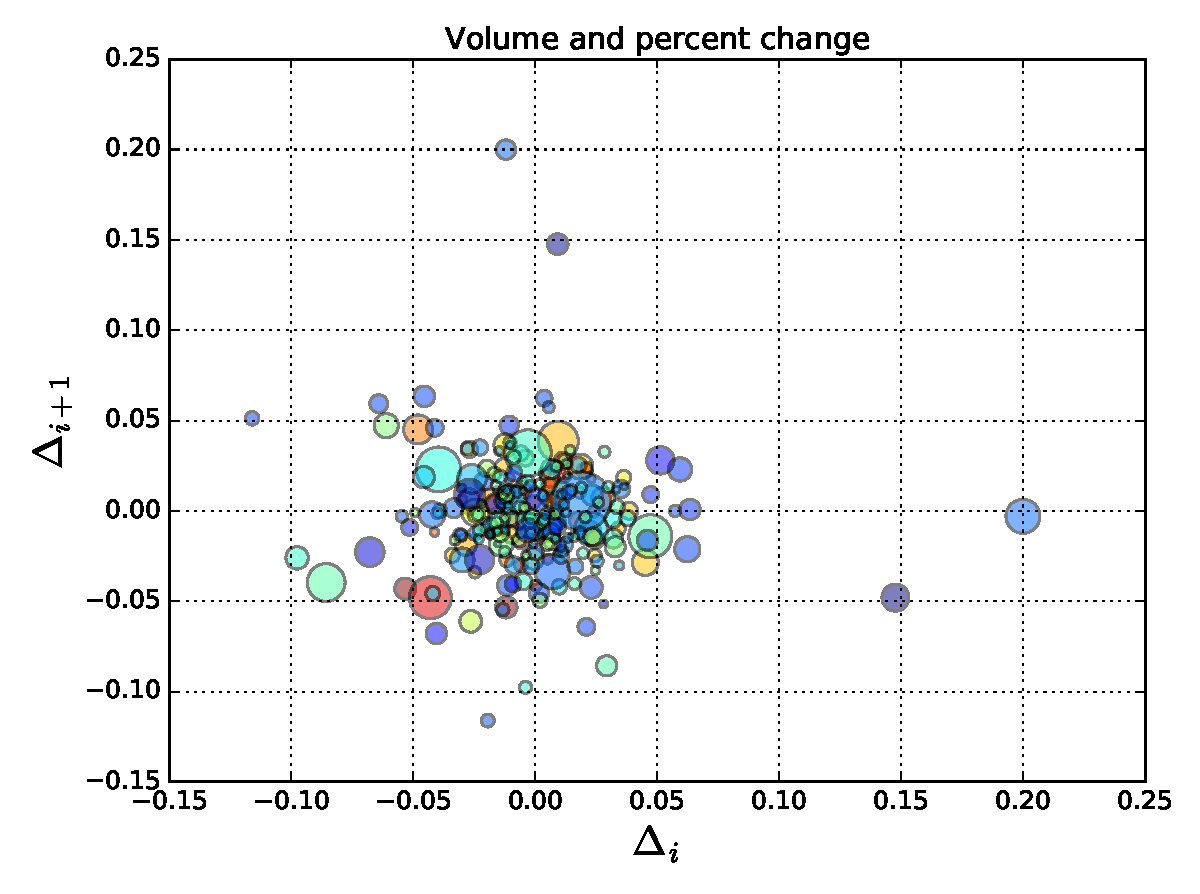
\includegraphics[width=15cm]{tabular-caption}
        \caption{一副图像}
    \end{center}
\end{figure}
